\documentclass{article}

\usepackage[landscape,margin={1in}]{geometry}
\usepackage{musicography}

\usepackage{tikz}

\usetikzlibrary{calc}

\newcommand{\myFlFl}{\raisebox{0.2ex}{\musDoubleFlat}}
\newcommand{\myFl}{\raisebox{0.2ex}{\musFlat}}
\newcommand{\mySh}{\raisebox{0.4ex}{\musSharp}}
\newcommand{\myShSh}{\raisebox{0.4ex}{\musDoubleSharp}}

\begin{document}
\pagestyle{empty}

%%%%%%%%%%%%%%%%%%%%%%%%%%%%%%%%%%%%%%%%%%%%%%%%%%%%%%%%%%%%%%%%%%%%%%%%

% Basic US keyboard layout

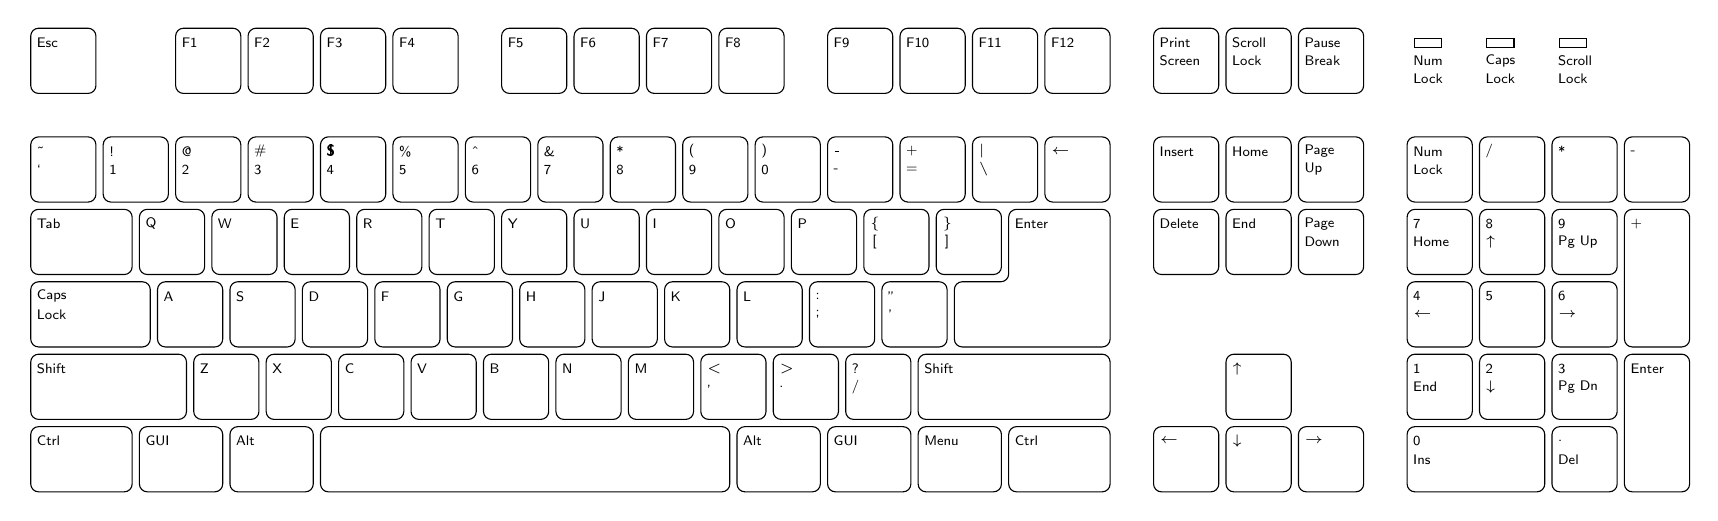
\begin{tikzpicture}[scale=0.23]
  % first row
  \foreach \xa/\xb/\ta/\tb in
    {0/4/Esc/{},
     8/12/F1/{},12/16/F2/{},16/20/F3/{},20/24/F4/{},
     26/30/F5/{},30/34/F6/{},34/38/F7/{},38/42/F8/{},
     44/48/F9/{},48/52/F10/{},52/56/F11/{},56/60/F12/{},
     62/66/Print/Screen,66/70/Scroll/Lock,70/74/Pause/Break} {
    \draw[rounded corners={1mm}]
      ($(\xa,22)+(0.2,0.2)$) rectangle ($(\xb,26)+(-0.2,-0.2)$);
    \node[anchor=west] at ($(\xa,26)+(0,-1)$) {\tiny\textsf{\ta}};
    \node[anchor=west] at ($(\xa,26)+(0,-2)$) {\tiny\textsf{\tb}};
  }
  % LEDs
  \foreach \x/\t in {76/Num,80/Caps,84/Scroll} {
    \draw (\x+0.6,24.75) rectangle (\x+2.1,25.25);
    \node[anchor=west] at ($(\x,26)+(0,-2)$) {\tiny\textsf{\t}};
    \node[anchor=west] at ($(\x,26)+(0,-3)$) {\tiny\textsf{Lock}};
  }
  % second row
  \foreach \xa/\xb/\ta/\tb in
    {0/4/{\textasciitilde}/{`},4/8/!/1,8/12/@/2,12/16/\#/3,
     16/20/\$/4,20/24/\%/5,24/28/\textasciicircum/6,28/32/\&/7,
     32/36/*/8,36/40/(/9,40/44/)/0,44/48/\textunderscore/-,
     48/52/+/=,52/56/{$\vert$}/\textbackslash,56/60/{$\leftarrow$}/{},
     62/66/Insert/{},66/70/Home/{},70/74/Page/Up,
     76/80/Num/Lock,80/84/{/}/{},84/88/*/{},88/92/-/{}} {
    \draw[rounded corners={1mm}]
      ($(\xa,16)+(0.2,0.2)$) rectangle ($(\xb,20)+(-0.2,-0.2)$);
    \node[anchor=west] at ($(\xa,20)+(0,-1)$) {\tiny\textsf{\ta}};
    \node[anchor=west] at ($(\xa,20)+(0,-2)$) {\tiny\textsf{\tb}};
  }
  % third row
  \foreach \xa/\xb/\ta/\tb in
    {0/6/Tab/{},6/10/Q/{},10/14/W/{},14/18/E/{},
     18/22/R/{},22/26/T/{},26/30/Y/{},30/34/U/{},
     34/38/I/{},38/42/O/{},42/46/P/{},46/50/{\{}/{\,[},
     50/54/{\}}/{\,]},
     62/66/Delete/{},66/70/End/{},70/74/Page/Down,
     76/80/7/Home,80/84/8/{$\uparrow$},84/88/9/Pg Up} {
    \draw[rounded corners={1mm}]
      ($(\xa,12)+(0.2,0.2)$) rectangle ($(\xb,16)+(-0.2,-0.2)$);
    \node[anchor=west] at ($(\xa,16)+(0,-1)$) {\tiny\textsf{\ta}};
    \node[anchor=west] at ($(\xa,16)+(0,-2)$) {\tiny\textsf{\tb}};
  }
  % keys that span third and fourth rows
  \draw[rounded corners={1mm}]
    ($(51,8)+(0.2,0.2)$) -- ($(51,12)+(0.2,-0.2)$) --
    ($(54,12)+(0.2,-0.2)$) -- ($(54,16)+(0.2,-0.2)$) --
    ($(60,16)+(-0.2,-0.2)$) -- ($(60,8)+(-0.2,0.2)$) --cycle;
  \node[anchor=west] at ($(54,16)+(0,-1)$) {\tiny\textsf{Enter}};
  \draw[rounded corners={1mm}]
    ($(88,8)+(0.2,0.2)$) rectangle ($(92,16)+(-0.2,-0.2)$);
  \node[anchor=west] at ($(88,16)+(0,-1)$) {\tiny\textsf{+}};
  % fourth row
  \foreach \xa/\xb/\ta/\tb in
    {0/7/Caps/Lock,7/11/A/{},11/15/S/{},15/19/D/{},
     19/23/F/{},23/27/G/{},27/31/H/{},31/35/J/{},
     35/39/K/{},39/43/L/{},43/47/:/;,47/51/{''}/{'},
     76/80/4/{$\leftarrow$},80/84/5/{},84/88/6/{$\rightarrow$}} {
    \draw[rounded corners={1mm}]
      ($(\xa,8)+(0.2,0.2)$) rectangle ($(\xb,12)+(-0.2,-0.2)$);
    \node[anchor=west] at ($(\xa,12)+(0,-1)$) {\tiny\textsf{\ta}};
    \node[anchor=west] at ($(\xa,12)+(0,-2)$) {\tiny\textsf{\tb}};
  }
  % fifth row
  \foreach \xa/\xb/\ta/\tb in
    {0/9/Shift/{},9/13/Z/{},13/17/X/{},17/21/C/{},
     21/25/V/{},25/29/B/{},29/33/N/{},33/37/M/{},
     37/41/{$<$}/{,},41/45/{$>$}/.,45/49/?/{/},49/60/Shift/{},
     66/70/{$\uparrow$}/{},
     76/80/1/End,80/84/2/{$\downarrow$},84/88/3/Pg Dn} {
    \draw[rounded corners={1mm}]
      ($(\xa,4)+(0.2,0.2)$) rectangle ($(\xb,8)+(-0.2,-0.2)$);
    \node[anchor=west] at ($(\xa,8)+(0,-1)$) {\tiny\textsf{\ta}};
    \node[anchor=west] at ($(\xa,8)+(0,-2)$) {\tiny\textsf{\tb}};
  }
  % keys that span fifth and sixth rows
  \draw[rounded corners={1mm}]
    ($(88,0)+(0.2,0.2)$) rectangle ($(92,8)+(-0.2,-0.2)$);
  \node[anchor=west] at ($(88,8)+(0,-1)$) {\tiny\textsf{Enter}};
  % sixth row
  \foreach \xa/\xb/\ta/\tb in
    {0/6/Ctrl/{},6/11/GUI/{},11/16/Alt/{},16/39/{}/{},
     39/44/Alt/{},44/49/GUI/{},49/54/Menu/{},54/60/Ctrl/{},
     62/66/{$\leftarrow$}/{},66/70/{$\downarrow$}/{},70/74/{$\rightarrow$}/{},
     76/84/0/Ins,84/88/./Del} {
    \draw[rounded corners={1mm}]
      ($(\xa,0)+(0.2,0.2)$) rectangle ($(\xb,4)+(-0.2,-0.2)$);
    \node[anchor=west] at ($(\xa,4)+(0,-1)$) {\tiny\textsf{\ta}};
    \node[anchor=west] at ($(\xa,4)+(0,-2)$) {\tiny\textsf{\tb}};
  }
\end{tikzpicture}

%%%%%%%%%%%%%%%%%%%%%%%%%%%%%%%%%%%%%%%%%%%%%%%%%%%%%%%%%%%%%%%%%%%%%%%%

% Basic ISO keyboard layout

\vspace{1cm}

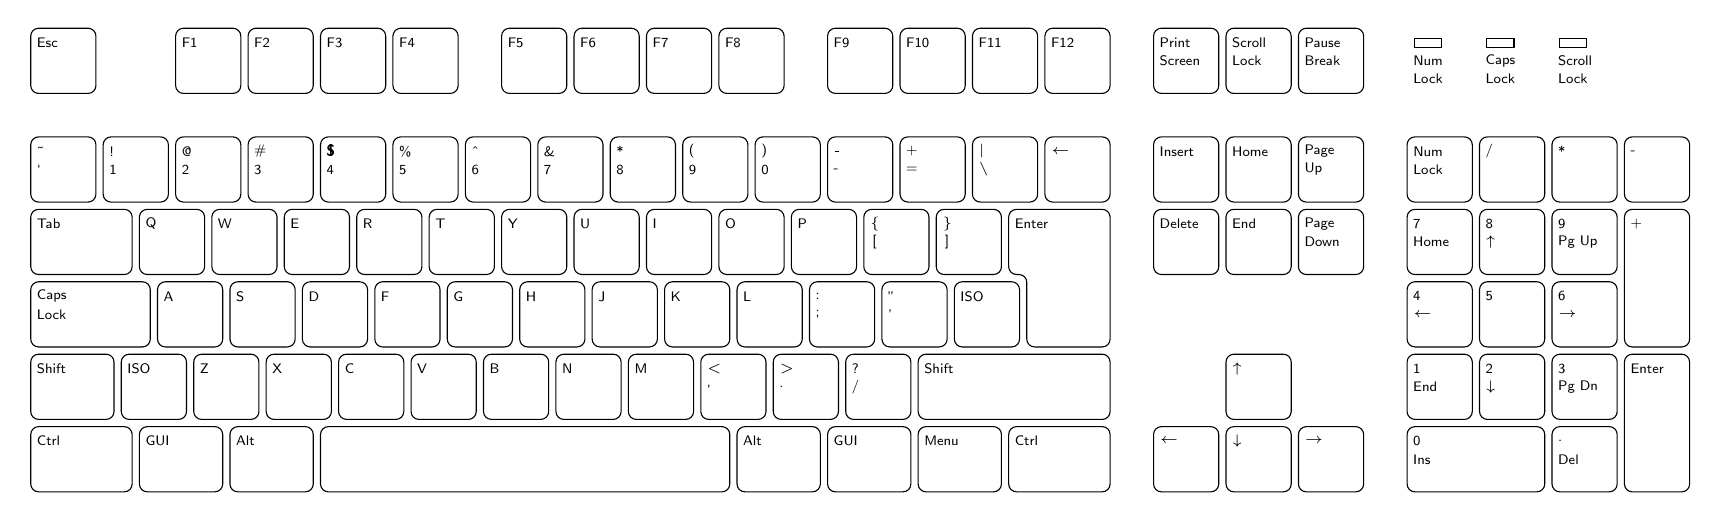
\begin{tikzpicture}[scale=0.23]
  % first row
  \foreach \xa/\xb/\ta/\tb in
    {0/4/Esc/{},
     8/12/F1/{},12/16/F2/{},16/20/F3/{},20/24/F4/{},
     26/30/F5/{},30/34/F6/{},34/38/F7/{},38/42/F8/{},
     44/48/F9/{},48/52/F10/{},52/56/F11/{},56/60/F12/{},
     62/66/Print/Screen,66/70/Scroll/Lock,70/74/Pause/Break} {
    \draw[rounded corners={1mm}]
      ($(\xa,22)+(0.2,0.2)$) rectangle ($(\xb,26)+(-0.2,-0.2)$);
    \node[anchor=west] at ($(\xa,26)+(0,-1)$) {\tiny\textsf{\ta}};
    \node[anchor=west] at ($(\xa,26)+(0,-2)$) {\tiny\textsf{\tb}};
  }
  % LEDs
  \foreach \x/\t in {76/Num,80/Caps,84/Scroll} {
    \draw (\x+0.6,24.75) rectangle (\x+2.1,25.25);
    \node[anchor=west] at ($(\x,26)+(0,-2)$) {\tiny\textsf{\t}};
    \node[anchor=west] at ($(\x,26)+(0,-3)$) {\tiny\textsf{Lock}};
  }
  % second row
  \foreach \xa/\xb/\ta/\tb in
    {0/4/{\textasciitilde}/{`},4/8/!/1,8/12/@/2,12/16/\#/3,
     16/20/\$/4,20/24/\%/5,24/28/\textasciicircum/6,28/32/\&/7,
     32/36/*/8,36/40/(/9,40/44/)/0,44/48/\textunderscore/-,
     48/52/+/=,52/56/{$\vert$}/\textbackslash,56/60/{$\leftarrow$}/{},
     62/66/Insert/{},66/70/Home/{},70/74/Page/Up,
     76/80/Num/Lock,80/84/{/}/{},84/88/*/{},88/92/-/{}} {
    \draw[rounded corners={1mm}]
      ($(\xa,16)+(0.2,0.2)$) rectangle ($(\xb,20)+(-0.2,-0.2)$);
    \node[anchor=west] at ($(\xa,20)+(0,-1)$) {\tiny\textsf{\ta}};
    \node[anchor=west] at ($(\xa,20)+(0,-2)$) {\tiny\textsf{\tb}};
  }
  % third row
  \foreach \xa/\xb/\ta/\tb in
    {0/6/Tab/{},6/10/Q/{},10/14/W/{},14/18/E/{},
     18/22/R/{},22/26/T/{},26/30/Y/{},30/34/U/{},
     34/38/I/{},38/42/O/{},42/46/P/{},46/50/{\{}/{\,[},
     50/54/{\}}/{\,]},
     62/66/Delete/{},66/70/End/{},70/74/Page/Down,
     76/80/7/Home,80/84/8/{$\uparrow$},84/88/9/Pg Up} {
    \draw[rounded corners={1mm}]
      ($(\xa,12)+(0.2,0.2)$) rectangle ($(\xb,16)+(-0.2,-0.2)$);
    \node[anchor=west] at ($(\xa,16)+(0,-1)$) {\tiny\textsf{\ta}};
    \node[anchor=west] at ($(\xa,16)+(0,-2)$) {\tiny\textsf{\tb}};
  }
  % keys that span third and fourth rows
  \draw[rounded corners={1mm}]
    ($(55,8)+(0.2,0.2)$) -- ($(55,12)+(0.2,0.2)$) --
    ($(54,12)+(0.2,0.2)$) -- ($(54,16)+(0.2,-0.2)$) --
    ($(60,16)+(-0.2,-0.2)$) -- ($(60,8)+(-0.2,0.2)$) --cycle;
  \node[anchor=west] at ($(54,16)+(0,-1)$) {\tiny\textsf{Enter}};
  \draw[rounded corners={1mm}]
    ($(88,8)+(0.2,0.2)$) rectangle ($(92,16)+(-0.2,-0.2)$);
  \node[anchor=west] at ($(88,16)+(0,-1)$) {\tiny\textsf{+}};
  % fourth row
  \foreach \xa/\xb/\ta/\tb in
    {0/7/Caps/Lock,7/11/A/{},11/15/S/{},15/19/D/{},
     19/23/F/{},23/27/G/{},27/31/H/{},31/35/J/{},
     35/39/K/{},39/43/L/{},43/47/:/;,47/51/{''}/{'},
     51/55/ISO/{},
     76/80/4/{$\leftarrow$},80/84/5/{},84/88/6/{$\rightarrow$}} {
    \draw[rounded corners={1mm}]
      ($(\xa,8)+(0.2,0.2)$) rectangle ($(\xb,12)+(-0.2,-0.2)$);
    \node[anchor=west] at ($(\xa,12)+(0,-1)$) {\tiny\textsf{\ta}};
    \node[anchor=west] at ($(\xa,12)+(0,-2)$) {\tiny\textsf{\tb}};
  }
  % fifth row
  \foreach \xa/\xb/\ta/\tb in
    {0/5/Shift/{},5/9/ISO/{},9/13/Z/{},13/17/X/{},17/21/C/{},
     21/25/V/{},25/29/B/{},29/33/N/{},33/37/M/{},
     37/41/{$<$}/{,},41/45/{$>$}/.,45/49/?/{/},49/60/Shift/{},
     66/70/{$\uparrow$}/{},
     76/80/1/End,80/84/2/{$\downarrow$},84/88/3/Pg Dn} {
    \draw[rounded corners={1mm}]
      ($(\xa,4)+(0.2,0.2)$) rectangle ($(\xb,8)+(-0.2,-0.2)$);
    \node[anchor=west] at ($(\xa,8)+(0,-1)$) {\tiny\textsf{\ta}};
    \node[anchor=west] at ($(\xa,8)+(0,-2)$) {\tiny\textsf{\tb}};
  }
  % keys that span fifth and sixth rows
  \draw[rounded corners={1mm}]
    ($(88,0)+(0.2,0.2)$) rectangle ($(92,8)+(-0.2,-0.2)$);
  \node[anchor=west] at ($(88,8)+(0,-1)$) {\tiny\textsf{Enter}};
  % sixth row
  \foreach \xa/\xb/\ta/\tb in
    {0/6/Ctrl/{},6/11/GUI/{},11/16/Alt/{},16/39/{}/{},
     39/44/Alt/{},44/49/GUI/{},49/54/Menu/{},54/60/Ctrl/{},
     62/66/{$\leftarrow$}/{},66/70/{$\downarrow$}/{},70/74/{$\rightarrow$}/{},
     76/84/0/Ins,84/88/./Del} {
    \draw[rounded corners={1mm}]
      ($(\xa,0)+(0.2,0.2)$) rectangle ($(\xb,4)+(-0.2,-0.2)$);
    \node[anchor=west] at ($(\xa,4)+(0,-1)$) {\tiny\textsf{\ta}};
    \node[anchor=west] at ($(\xa,4)+(0,-2)$) {\tiny\textsf{\tb}};
  }
\end{tikzpicture}

%%%%%%%%%%%%%%%%%%%%%%%%%%%%%%%%%%%%%%%%%%%%%%%%%%%%%%%%%%%%%%%%%%%%%%%%

% ISO piano-style

\vspace{1cm}

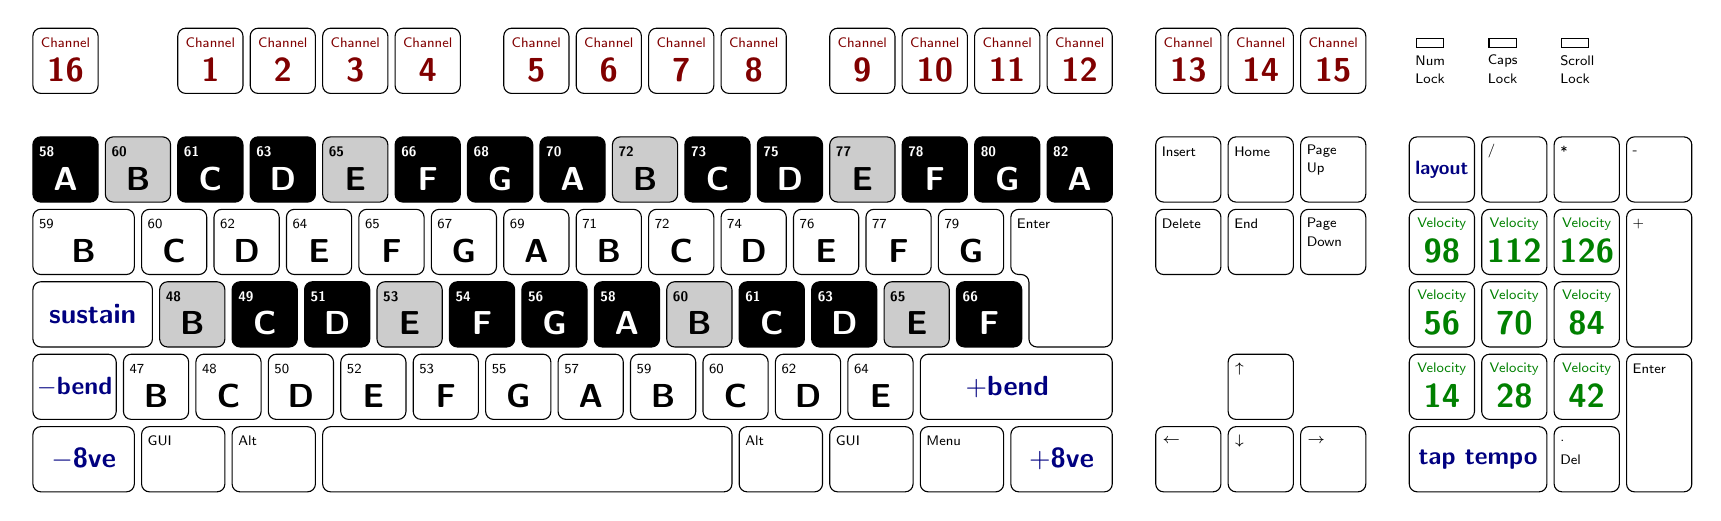
\begin{tikzpicture}[scale=0.23]
  % first row
  \foreach \xa/\xb/\tb in
    {0/4/16,
     8/12/1,12/16/2,16/20/3,20/24/4,
     26/30/5,30/34/6,34/38/7,38/42/8,
     44/48/9,48/52/10,52/56/11,56/60/12,
     62/66/13,66/70/14,70/74/15} {
    \draw[rounded corners={1mm}]
      ($(\xa,22)+(0.2,0.2)$) rectangle ($(\xb,26)+(-0.2,-0.2)$);
    \node[red!50!black] at ($(\xa,26)+(2,-1)$)
      {\tiny\textsf{Channel}};
    \node[red!50!black] at ($(\xa,22)+(2,1.5)$) {\large\bf\textsf{\tb}};
  }
  % LEDs
  \foreach \x/\t in {76/Num,80/Caps,84/Scroll} {
    \draw (\x+0.6,24.75) rectangle (\x+2.1,25.25);
    \node[anchor=west] at ($(\x,26)+(0,-2)$) {\tiny\textsf{\t}};
    \node[anchor=west] at ($(\x,26)+(0,-3)$) {\tiny\textsf{Lock}};
  }
  % second row, black note keys
  \foreach \xa/\xb/\ta/\tb in
    {0/4/58/{A\mySh},8/12/61/{C\mySh},12/16/63/{D\mySh},
     20/24/66/{F\mySh},24/28/68/{G\mySh},28/32/70/{A\mySh},
     36/40/73/{C\mySh},40/44/75/{D\mySh},48/52/78/{F\mySh},
     52/56/80/{G\mySh},56/60/82/{A\mySh}} {
    \draw[rounded corners={1mm},fill=black]
      ($(\xa,16)+(0.2,0.2)$) rectangle ($(\xb,20)+(-0.2,-0.2)$);
    \node[anchor=west,white] at ($(\xa,20)+(0,-1)$) {\tiny\bf\textsf{\ta}};
    \node[white] at ($(\xa,16)+(2,1.5)$) {\large\bf\textsf{\tb}};
  }
  % second row, skipped keys
  \foreach \xa/\xb/\ta/\tb in
    {4/8/60/{B\mySh},16/20/65/{E\mySh},32/36/72/{B\mySh},44/48/77/{E\mySh}} {
    \draw[rounded corners={1mm},fill=black!20!white]
      ($(\xa,16)+(0.2,0.2)$) rectangle ($(\xb,20)+(-0.2,-0.2)$);
    \node[anchor=west] at ($(\xa,20)+(0,-1)$) {\tiny\bf\textsf{\ta}};
    \node at ($(\xa,16)+(2,1.5)$) {\large\bf\textsf{\tb}};
  }
  % second row, non-note keys
  \foreach \xa/\xb/\ta/\tb in
    {62/66/Insert/{},66/70/Home/{},70/74/Page/Up,
     76/80/{}/{},80/84/{/}/{},84/88/*/{},88/92/-/{}} {
    \draw[rounded corners={1mm}]
      ($(\xa,16)+(0.2,0.2)$) rectangle ($(\xb,20)+(-0.2,-0.2)$);
    \node[anchor=west] at ($(\xa,20)+(0,-1)$) {\tiny\textsf{\ta}};
    \node[anchor=west] at ($(\xa,20)+(0,-2)$) {\tiny\textsf{\tb}};
  }
  % third row, white note keys
  \foreach \xa/\xb/\ta/\tb in
    {0/6/59/B,6/10/60/C,10/14/62/D,14/18/64/E,
     18/22/65/F,22/26/67/G,26/30/69/A,30/34/71/B,
     34/38/72/C,38/42/74/D,42/46/76/E,46/50/77/F,
     50/54/79/G} {
    \draw[rounded corners={1mm}]
      ($(\xa,12)+(0.2,0.2)$) rectangle ($(\xb,16)+(-0.2,-0.2)$);
    \node[anchor=west] at ($(\xa,16)+(0,-1)$) {\tiny\textsf{\ta}};
    \node at ($(\xa,12+1.5)!0.5!(\xb,12+1.5)$) {\large\bf\textsf{\tb}};
  }
  % third row, non-note keys
  \foreach \xa/\xb/\ta/\tb in
    {62/66/Delete/{},66/70/End/{},70/74/Page/Down} {
    \draw[rounded corners={1mm}]
      ($(\xa,12)+(0.2,0.2)$) rectangle ($(\xb,16)+(-0.2,-0.2)$);
    \node[anchor=west] at ($(\xa,16)+(0,-1)$) {\tiny\textsf{\ta}};
    \node[anchor=west] at ($(\xa,16)+(0,-2)$) {\tiny\textsf{\tb}};
  }
  % keys that span third and fourth rows
  \draw[rounded corners={1mm}]
    ($(55,8)+(0.2,0.2)$) -- ($(55,12)+(0.2,0.2)$) --
    ($(54,12)+(0.2,0.2)$) -- ($(54,16)+(0.2,-0.2)$) --
    ($(60,16)+(-0.2,-0.2)$) -- ($(60,8)+(-0.2,0.2)$) --cycle;
  \node[anchor=west] at ($(54,16)+(0,-1)$) {\tiny\textsf{Enter}};
  \draw[rounded corners={1mm}]
    ($(88,8)+(0.2,0.2)$) rectangle ($(92,16)+(-0.2,-0.2)$);
  \node[anchor=west] at ($(88,16)+(0,-1)$) {\tiny\textsf{+}};
  % fourth row, black note keys
  \foreach \xa/\xb/\ta/\tb in
    {11/15/49/{C\mySh},15/19/51/{D\mySh},
     23/27/54/{F\mySh},27/31/56/{G\mySh},31/35/58/{A\mySh},
     39/43/61/{C\mySh},43/47/63/{D\mySh},
     51/55/66/{F\mySh}} {
    \draw[rounded corners={1mm}, fill=black]
      ($(\xa,8)+(0.2,0.2)$) rectangle ($(\xb,12)+(-0.2,-0.2)$);
    \node[anchor=west,white] at ($(\xa,12)+(0,-1)$) {\tiny\bf\textsf{\ta}};
    \node[white] at ($(\xa,8)+(2,1.5)$) {\large\bf\textsf{\tb}};
  }
  % fourth row, skipped keys
  \foreach \xa/\xb/\ta/\tb in
    {7/11/48/{B\mySh},
     19/23/53/{E\mySh},
     35/39/60/{B\mySh},47/51/65/{E\mySh}} {
    \draw[rounded corners={1mm},fill=black!20!white]
      ($(\xa,8)+(0.2,0.2)$) rectangle ($(\xb,12)+(-0.2,-0.2)$);
    \node[anchor=west] at ($(\xa,12)+(0,-1)$) {\tiny\bf\textsf{\ta}};
    \node at ($(\xa,8)+(2,1.5)$) {\large\bf\textsf{\tb}};
  }
  % fourth row, non-note keys
  \foreach \xa/\xb/\ta/\tb in
    {0/7/{}/{}} {
    \draw[rounded corners={1mm}]
      ($(\xa,8)+(0.2,0.2)$) rectangle ($(\xb,12)+(-0.2,-0.2)$);
    \node[anchor=west] at ($(\xa,12)+(0,-1)$) {\tiny\textsf{\ta}};
    \node[anchor=west] at ($(\xa,12)+(0,-2)$) {\tiny\textsf{\tb}};
  }
  % fifth row, white note keys
  \foreach \xa/\xb/\ta/\tb in
    {5/9/47/B,9/13/48/C,13/17/50/D,17/21/52/E,
     21/25/53/F,25/29/55/G,29/33/57/A,33/37/59/B,
     37/41/60/C,41/45/62/D,45/49/64/E} {
    \draw[rounded corners={1mm}]
      ($(\xa,4)+(0.2,0.2)$) rectangle ($(\xb,8)+(-0.2,-0.2)$);
    \node[anchor=west] at ($(\xa,8)+(0,-1)$) {\tiny\textsf{\ta}};
    \node at ($(\xa,4+1.5)!0.5!(\xb,4+1.5)$) {\large\bf\textsf{\tb}};
  }
  % fifth row, non-note keys
  \foreach \xa/\xb/\ta/\tb in
    {0/5/{}/{},49/60/{}/{},
     66/70/{$\uparrow$}/{}} {
    \draw[rounded corners={1mm}]
      ($(\xa,4)+(0.2,0.2)$) rectangle ($(\xb,8)+(-0.2,-0.2)$);
    \node[anchor=west] at ($(\xa,8)+(0,-1)$) {\tiny\textsf{\ta}};
    \node[anchor=west] at ($(\xa,8)+(0,-2)$) {\tiny\textsf{\tb}};
  }
  % keys that span fifth and sixth rows
  \draw[rounded corners={1mm}]
    ($(88,0)+(0.2,0.2)$) rectangle ($(92,8)+(-0.2,-0.2)$);
  \node[anchor=west] at ($(88,8)+(0,-1)$) {\tiny\textsf{Enter}};
  % sixth row
  \foreach \xa/\xb/\ta/\tb in
    {0/6/{}/{},6/11/GUI/{},11/16/Alt/{},16/39/{}/{},
     39/44/Alt/{},44/49/GUI/{},49/54/Menu/{},54/60/{}/{},
     62/66/{$\leftarrow$}/{},66/70/{$\downarrow$}/{},70/74/{$\rightarrow$}/{},
     76/84/{}/{},84/88/./Del} {
    \draw[rounded corners={1mm}]
      ($(\xa,0)+(0.2,0.2)$) rectangle ($(\xb,4)+(-0.2,-0.2)$);
    \node[anchor=west] at ($(\xa,4)+(0,-1)$) {\tiny\textsf{\ta}};
    \node[anchor=west] at ($(\xa,4)+(0,-2)$) {\tiny\textsf{\tb}};
  }
  % keypad numerals
  \foreach \x/\y/\t in {76/4/14,80/4/28,84/4/42,76/8/56,80/8/70,
    84/8/84,76/12/98,80/12/112,84/12/126} {
    \draw[rounded corners={1mm}]
      ($(\x,\y)+(0.2,0.2)$) rectangle ($(\x+4,\y+4)+(-0.2,-0.2)$);
    \node[green!50!black] at ($(\x,\y)+(2,3)$)
      {\tiny\textsf{Velocity}};
    \node[green!50!black] at ($(\x,\y)+(2,1.5)$) {\large\bf\textsf{\t}};
  }
  % additional key labels
  \node[blue!50!black] at (3.5,10) {\bf\textsf{sustain}};
  \node[blue!50!black] at (2.5,6) {\small\bf\textsf{$-$bend}};
  \node[blue!50!black] at (3,2) {\bf\textsf{$-$8ve}};
  \node[blue!50!black] at (54,6) {\bf\textsf{$+$bend}};
  \node[blue!50!black] at (57,2) {\bf\textsf{$+$8ve}};
  \node[blue!50!black] at (78,18) {\scriptsize\bf\textsf{layout}};
  \node[blue!50!black] at (80,2) {\small\bf\textsf{tap tempo}};
\end{tikzpicture}

%%%%%%%%%%%%%%%%%%%%%%%%%%%%%%%%%%%%%%%%%%%%%%%%%%%%%%%%%%%%%%%%%%%%%%%%

% ISO Wicki-Hayden

\vspace{1cm}

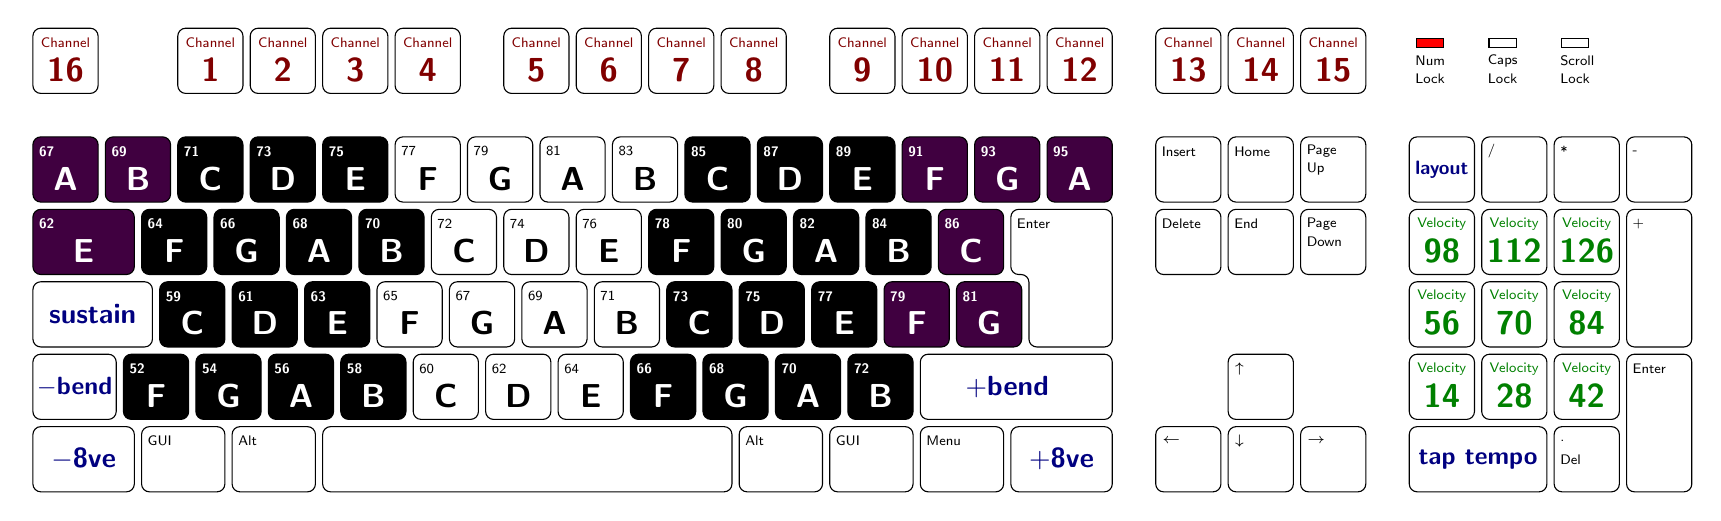
\begin{tikzpicture}[scale=0.23]
  % first row
  \foreach \xa/\xb/\tb in
    {0/4/16,
     8/12/1,12/16/2,16/20/3,20/24/4,
     26/30/5,30/34/6,34/38/7,38/42/8,
     44/48/9,48/52/10,52/56/11,56/60/12,
     62/66/13,66/70/14,70/74/15} {
    \draw[rounded corners={1mm}]
      ($(\xa,22)+(0.2,0.2)$) rectangle ($(\xb,26)+(-0.2,-0.2)$);
    \node[red!50!black] at ($(\xa,26)+(2,-1)$)
      {\tiny\textsf{Channel}};
    \node[red!50!black] at ($(\xa,22)+(2,1.5)$) {\large\bf\textsf{\tb}};
  }
  % LEDs
  \foreach \x/\t in {80/Caps,84/Scroll} {
    \draw (\x+0.6,24.75) rectangle (\x+2.1,25.25);
    \node[anchor=west] at ($(\x,26)+(0,-2)$) {\tiny\textsf{\t}};
    \node[anchor=west] at ($(\x,26)+(0,-3)$) {\tiny\textsf{Lock}};
  }
  \draw[fill=red] (76+0.6,24.75) rectangle (76+2.1,25.25);
  \node[anchor=west] at ($(76,26)+(0,-2)$) {\tiny\textsf{Num}};
  \node[anchor=west] at ($(76,26)+(0,-3)$) {\tiny\textsf{Lock}};
  % second row, purple note keys
  \foreach \xa/\xb/\ta/\tb in
    {0/4/67/{A\myFlFl},4/8/69/{B\myFlFl},48/52/91/{F\myShSh},
     52/56/93/{G\myShSh},56/60/95/{A\myShSh}} {
    \draw[rounded corners={1mm},fill=red!50!blue!50!black]
      ($(\xa,16)+(0.2,0.2)$) rectangle ($(\xb,20)+(-0.2,-0.2)$);
    \node[anchor=west,white] at ($(\xa,20)+(0,-1)$) {\tiny\bf\textsf{\ta}};
    \node[white] at ($(\xa,16)+(2,1.5)$) {\large\bf\textsf{\tb}};
  }
  % second row, black note keys
  \foreach \xa/\xb/\ta/\tb in
    {8/12/71/{C\myFl},12/16/73/{D\myFl},16/20/75/{E\myFl},
     36/40/85/{C\mySh},40/44/87/{D\mySh},44/48/89/{E\mySh}} {
    \draw[rounded corners={1mm},fill=black]
      ($(\xa,16)+(0.2,0.2)$) rectangle ($(\xb,20)+(-0.2,-0.2)$);
    \node[anchor=west,white] at ($(\xa,20)+(0,-1)$) {\tiny\bf\textsf{\ta}};
    \node[white] at ($(\xa,16)+(2,1.5)$) {\large\bf\textsf{\tb}};
  }
  % second row, white note keys
  \foreach \xa/\xb/\ta/\tb in
    {20/24/77/F,24/28/79/G,28/32/81/A,32/36/83/B} {
    \draw[rounded corners={1mm}]
      ($(\xa,16)+(0.2,0.2)$) rectangle ($(\xb,20)+(-0.2,-0.2)$);
    \node[anchor=west] at ($(\xa,20)+(0,-1)$) {\tiny\textsf{\ta}};
    \node at ($(\xa,16)+(2,1.5)$) {\large\bf\textsf{\tb}};
  }
  % second row, non-note keys
  \foreach \xa/\xb/\ta/\tb in
    {62/66/Insert/{},66/70/Home/{},70/74/Page/Up,
     76/80/{}/{},80/84/{/}/{},84/88/*/{},88/92/-/{}} {
    \draw[rounded corners={1mm}]
      ($(\xa,16)+(0.2,0.2)$) rectangle ($(\xb,20)+(-0.2,-0.2)$);
    \node[anchor=west] at ($(\xa,20)+(0,-1)$) {\tiny\textsf{\ta}};
    \node[anchor=west] at ($(\xa,20)+(0,-2)$) {\tiny\textsf{\tb}};
  }
  % third row, purple note keys
  \foreach \xa/\xb/\ta/\tb in
    {0/6/62/{E\myFlFl},50/54/86/{C\myShSh}} {
    \draw[rounded corners={1mm},fill=red!50!blue!50!black]
      ($(\xa,12)+(0.2,0.2)$) rectangle ($(\xb,16)+(-0.2,-0.2)$);
    \node[anchor=west,white] at ($(\xa,16)+(0,-1)$) {\tiny\bf\textsf{\ta}};
    \node[white] at ($(\xa,12+1.5)!0.5!(\xb,12+1.5)$) {\large\bf\textsf{\tb}};
  }
  % third row, black note keys
  \foreach \xa/\xb/\ta/\tb in
    {6/10/64/{F\myFl},10/14/66/{G\myFl},14/18/68/{A\myFl},18/22/70/{B\myFl},
     34/38/78/{F\mySh},38/42/80/{G\mySh},42/46/82/{A\mySh},46/50/84/{B\mySh}} {
    \draw[rounded corners={1mm},fill=black]
      ($(\xa,12)+(0.2,0.2)$) rectangle ($(\xb,16)+(-0.2,-0.2)$);
    \node[anchor=west,white] at ($(\xa,16)+(0,-1)$) {\tiny\bf\textsf{\ta}};
    \node[white] at ($(\xa,12+1.5)!0.5!(\xb,12+1.5)$) {\large\bf\textsf{\tb}};
  }
  % third row, white note keys
  \foreach \xa/\xb/\ta/\tb in
    {22/26/72/C,26/30/74/D,30/34/76/E} {
    \draw[rounded corners={1mm}]
      ($(\xa,12)+(0.2,0.2)$) rectangle ($(\xb,16)+(-0.2,-0.2)$);
    \node[anchor=west] at ($(\xa,16)+(0,-1)$) {\tiny\textsf{\ta}};
    \node at ($(\xa,12+1.5)!0.5!(\xb,12+1.5)$) {\large\bf\textsf{\tb}};
  }
  % third row, non-note keys
  \foreach \xa/\xb/\ta/\tb in
    {62/66/Delete/{},66/70/End/{},70/74/Page/Down} {
    \draw[rounded corners={1mm}]
      ($(\xa,12)+(0.2,0.2)$) rectangle ($(\xb,16)+(-0.2,-0.2)$);
    \node[anchor=west] at ($(\xa,16)+(0,-1)$) {\tiny\textsf{\ta}};
    \node[anchor=west] at ($(\xa,16)+(0,-2)$) {\tiny\textsf{\tb}};
  }
  % keys that span third and fourth rows
  \draw[rounded corners={1mm}]
    ($(55,8)+(0.2,0.2)$) -- ($(55,12)+(0.2,0.2)$) --
    ($(54,12)+(0.2,0.2)$) -- ($(54,16)+(0.2,-0.2)$) --
    ($(60,16)+(-0.2,-0.2)$) -- ($(60,8)+(-0.2,0.2)$) --cycle;
  \node[anchor=west] at ($(54,16)+(0,-1)$) {\tiny\textsf{Enter}};
  \draw[rounded corners={1mm}]
    ($(88,8)+(0.2,0.2)$) rectangle ($(92,16)+(-0.2,-0.2)$);
  \node[anchor=west] at ($(88,16)+(0,-1)$) {\tiny\textsf{+}};
  % fourth row, purple note keys
  \foreach \xa/\xb/\ta/\tb in
    {47/51/79/{F\myShSh},51/55/81/{G\myShSh}} {
    \draw[rounded corners={1mm},fill=red!50!blue!50!black]
      ($(\xa,8)+(0.2,0.2)$) rectangle ($(\xb,12)+(-0.2,-0.2)$);
    \node[anchor=west,white] at ($(\xa,12)+(0,-1)$) {\tiny\bf\textsf{\ta}};
    \node[white] at ($(\xa,8+1.5)!0.5!(\xb,8+1.5)$) {\large\bf\textsf{\tb}};
  }
  % fourth row, black note keys
  \foreach \xa/\xb/\ta/\tb in
    {7/11/59/{C\myFl},11/15/61/{D\myFl},15/19/63/{E\myFl},
     35/39/73/{C\mySh},39/43/75/{D\mySh},43/47/77/{E\mySh}} {
    \draw[rounded corners={1mm},fill=black]
      ($(\xa,8)+(0.2,0.2)$) rectangle ($(\xb,12)+(-0.2,-0.2)$);
    \node[anchor=west,white] at ($(\xa,12)+(0,-1)$) {\tiny\bf\textsf{\ta}};
    \node[white] at ($(\xa,8+1.5)!0.5!(\xb,8+1.5)$) {\large\bf\textsf{\tb}};
  }
  % fourth row, white note keys
  \foreach \xa/\xb/\ta/\tb in
    {0/7/{}/{},19/23/65/F,23/27/67/G,27/31/69/A,31/35/71/B} {
    \draw[rounded corners={1mm}]
      ($(\xa,8)+(0.2,0.2)$) rectangle ($(\xb,12)+(-0.2,-0.2)$);
    \node[anchor=west] at ($(\xa,12)+(0,-1)$) {\tiny\textsf{\ta}};
    \node at ($(\xa,8+1.5)!0.5!(\xb,8+1.5)$) {\large\bf\textsf{\tb}};
  }
  % fifth row, black note keys
  \foreach \xa/\xb/\ta/\tb in
    {5/9/52/{F\myFl},9/13/54/{G\myFl},13/17/56/{A\myFl},17/21/58/{B\myFl},
     33/37/66/{F\mySh},37/41/68/{G\mySh},41/45/70/{A\mySh},45/49/72/{B\mySh}} {
    \draw[rounded corners={1mm},fill=black]
      ($(\xa,4)+(0.2,0.2)$) rectangle ($(\xb,8)+(-0.2,-0.2)$);
    \node[anchor=west,white] at ($(\xa,8)+(0,-1)$) {\tiny\bf\textsf{\ta}};
    \node[white] at ($(\xa,4+1.5)!0.5!(\xb,4+1.5)$) {\large\bf\textsf{\tb}};
  }
  % fifth row, white note keys
  \foreach \xa/\xb/\ta/\tb in
    {21/25/60/C,25/29/62/D,29/33/64/E} {
    \draw[rounded corners={1mm}]
      ($(\xa,4)+(0.2,0.2)$) rectangle ($(\xb,8)+(-0.2,-0.2)$);
    \node[anchor=west] at ($(\xa,8)+(0,-1)$) {\tiny\textsf{\ta}};
    \node at ($(\xa,4+1.5)!0.5!(\xb,4+1.5)$) {\large\bf\textsf{\tb}};
  }
  % fifth row, non-note keys
  \foreach \xa/\xb/\ta/\tb in
    {0/5/{}/{},49/60/{}/{},
     66/70/{$\uparrow$}/{}} {
    \draw[rounded corners={1mm}]
      ($(\xa,4)+(0.2,0.2)$) rectangle ($(\xb,8)+(-0.2,-0.2)$);
    \node[anchor=west] at ($(\xa,8)+(0,-1)$) {\tiny\textsf{\ta}};
    \node[anchor=west] at ($(\xa,8)+(0,-2)$) {\tiny\textsf{\tb}};
  }
  % keys that span fifth and sixth rows
  \draw[rounded corners={1mm}]
    ($(88,0)+(0.2,0.2)$) rectangle ($(92,8)+(-0.2,-0.2)$);
  \node[anchor=west] at ($(88,8)+(0,-1)$) {\tiny\textsf{Enter}};
  % sixth row
  \foreach \xa/\xb/\ta/\tb in
    {0/6/{}/{},6/11/GUI/{},11/16/Alt/{},16/39/{}/{},
     39/44/Alt/{},44/49/GUI/{},49/54/Menu/{},54/60/{}/{},
     62/66/{$\leftarrow$}/{},66/70/{$\downarrow$}/{},70/74/{$\rightarrow$}/{},
     76/84/{}/{},84/88/./Del} {
    \draw[rounded corners={1mm}]
      ($(\xa,0)+(0.2,0.2)$) rectangle ($(\xb,4)+(-0.2,-0.2)$);
    \node[anchor=west] at ($(\xa,4)+(0,-1)$) {\tiny\textsf{\ta}};
    \node[anchor=west] at ($(\xa,4)+(0,-2)$) {\tiny\textsf{\tb}};
  }
  % keypad numerals
  \foreach \x/\y/\t in {76/4/14,80/4/28,84/4/42,76/8/56,80/8/70,
    84/8/84,76/12/98,80/12/112,84/12/126} {
    \draw[rounded corners={1mm}]
      ($(\x,\y)+(0.2,0.2)$) rectangle ($(\x+4,\y+4)+(-0.2,-0.2)$);
    \node[green!50!black] at ($(\x,\y)+(2,3)$)
      {\tiny\textsf{Velocity}};
    \node[green!50!black] at ($(\x,\y)+(2,1.5)$) {\large\bf\textsf{\t}};
  }
  % additional key labels
  \node[blue!50!black] at (3.5,10) {\bf\textsf{sustain}};
  \node[blue!50!black] at (2.5,6) {\small\bf\textsf{$-$bend}};
  \node[blue!50!black] at (3,2) {\bf\textsf{$-$8ve}};
  \node[blue!50!black] at (54,6) {\bf\textsf{$+$bend}};
  \node[blue!50!black] at (57,2) {\bf\textsf{$+$8ve}};
  \node[blue!50!black] at (78,18) {\scriptsize\bf\textsf{layout}};
  \node[blue!50!black] at (80,2) {\small\bf\textsf{tap tempo}};
\end{tikzpicture}

\end{document}
